\documentclass[10pt,twocolumn,letterpaper]{article}

%%%%%%%%% PAPER TYPE  - PLEASE UPDATE FOR FINAL VERSION
\usepackage{cvpr}              % To produce the CAMERA-READY version
% \usepackage[review]{cvpr}      % To produce the REVIEW version
% \usepackage[pagenumbers]{cvpr} % To force page numbers, e.g. for an arXiv version

% Import additional packages in the preamble file, before hyperref
\usepackage[dvipsnames]{xcolor}
\newcommand{\red}[1]{{\color{red}#1}}
\newcommand{\todo}[1]{{\color{red}#1}}
\newcommand{\TODO}[1]{\textbf{\color{red}[TODO:#1]}}

% It is strongly recommended to use hyperref, especially for the review version.
% hyperref with option pagebackref eases the reviewers' job.
% Please disable hyperref *only* if you encounter grave issues, 
% e.g. with the file validation for the camera-ready version.
%
% If you comment hyperref and then uncomment it, you should delete *.aux before re-running LaTeX.
% (Or just hit 'q' on the first LaTeX run, let it finish, and you should be clear).
\definecolor{cvprblue}{rgb}{0.21,0.49,0.74}
\usepackage[pagebackref,breaklinks,colorlinks,citecolor=cvprblue]{hyperref}


%%%%%%%%% PAPER ID  - PLEASE UPDATE
\def\paperID{*****} % *** Enter the Paper ID here
\def\confName{CVPR}
\def\confYear{2024}

%%%%%%%%% TITLE - PLEASE UPDATE
\title{\ Bayesian Data Analysis using Monte Carlo Methods\ }

% \author{
%     Kshitiz Kumar\\
%     \texttt{ai22mtech02002@iith.ac.in} \and
%     Tanay Yadav\\
%     \texttt{ai20btech11026@iith.ac.in} \and
%     Tanmay Goyal\\
%     \texttt{ai20btech11021@iith.ac.in} \and
%     Tanmay Shah\\
%     \texttt{ee20btech11061@iith.ac.in}
% }

%%%%%%%% AUTHORS - PLEASE UPDATE
\author{Shreyas Wankhede\\
{\tt\small ai21btech11028@iith.ac.in}
% For a paper whose authors are all at the same institution,
% omit the following lines up until the closing ``}''.
% Additional authors and addresses can be added with ``\and'',
% just like the second author.
% To save space, use either the email address or home page, not both
\and
Pradeep Mundlik\\
{\tt\small ai21btech11022@iith.ac.in}
}


\begin{document}
\maketitle
\begin{abstract}
    This research investigates the application of Bayesian methods for probabilistic inference, specifically employing the Markov Chain Monte Carlo (MCMC) for data analysis. Bayesian approaches offer several advantages such as incorporation of prior knowledge, explicit uncertainty management, and the ease of assimilating new information, which is particularly useful in high-dimensional statistical models. Our study leverages MCMC to infer the parameters of interest in vehicular stopping distances by constructing a linear model to represent the relationship between a vehicle's speed and its stopping distance. We undertake a rigorous computational approach to address the challenges posed by numerical integration in high-dimensional spaces, presenting an effective strategy for sampling from complex posterior distributions.
\end{abstract}   

\section{Introduction}

Bayesian methods are currently experiencing an increase in popularity in the sciences as a means of probabilistic inference (Malakoff, 1999). Among their advantages are the ability to include prior information, the ease of incorporation into a formal decision analytic context, the explicit handling of uncertainty, and the straightforward ability to assimilate new information in contexts such as adaptive management. The Bayesian approach has been shown to be particularly useful for ecological models with poor parameter identifiability (Reichert and Omlin, 1997).

In a modelling application, Bayesian inference concerns the estimation of the values of $p$ unknown model parameters: $\boldsymbol{\theta} = (\theta_1, \ldots, \theta_p)$ about which there may be some prior beliefs. These prior beliefs can be expressed as a probability density function, $\pi(\boldsymbol{\theta})$, and may be interpreted as the probability placed on all possible parameter values before collecting any new data. The dependence of observations $\mathbf{D} = (d_1, \ldots, d_n)$ on the $p$ parameters can be expressed as the probability density function, $L(\mathbf{D} | \boldsymbol{\theta})$. This p.d.f is often referred to as the likelihood function and is used to update the prior beliefs on $\boldsymbol{\theta}$ to account for the new data, $\mathbf{D}$. This updating is performed using Bayes’ theorem which can be expressed:

\begin{equation}
\pi(\boldsymbol{\theta} | \mathbf{D}) = \frac{\pi(\mathbf{D} | \boldsymbol{\theta})\pi(\boldsymbol{\theta})}{\int \pi(\mathbf{D} | \boldsymbol{\theta})\pi(\boldsymbol{\theta}) d\boldsymbol{\theta}}
\end{equation}

where $\pi(\mathbf{D} | \boldsymbol{\theta})$ is called the posterior distribution and expresses the probability of the parameter values after observing the new data. Because the denominator in Eq. (1) is a normalizing constant, Bayes’ theorem is often expressed as:

\begin{equation}
\pi(\boldsymbol{\theta} | \mathbf{D}) \propto \pi(\mathbf{D} | \boldsymbol{\theta})\pi(\boldsymbol{\theta})
\end{equation}

indicating that the prior expectations are modified by the likelihood function to yield the posterior belief.

Once the posterior distribution is available, any features of $\boldsymbol{\theta}$, such as the marginal distributions or means and variances of the individual $\theta_i$, as well as the predictive distribution of future observations, require integrating over the posterior distribution. For example, the marginal posterior distribution of an individual $\theta_i$, can be calculated as:

\begin{equation}
\pi(\theta_i | \mathbf{D}) = \int \pi(\boldsymbol{\theta} | \mathbf{D}) d\boldsymbol{\theta}_{-i}
\end{equation}

where $\boldsymbol{\theta}_{-i}$ represents all $\theta$'s except $\theta_i$.

Most Bayesian inference problems can be succinctly expressed as the expectation of a function of interest, $g(\boldsymbol{\theta})$, evaluated over the posterior distribution:

\begin{equation}
E[g(\boldsymbol{\theta}) | \mathbf{D}] = \int \pi(\boldsymbol{\theta} | \mathbf{D})g(\boldsymbol{\theta}) d\boldsymbol{\theta}
\end{equation}

where $E$ denotes the expectation operator.

 
\section{Monte Carlo Approach}\label{sec:Monte_Carlo}
The Monte Carlo method is a broad class of computational algorithms that rely on repeated random sampling to obtain numerical results. Typically used in scenarios where exact solutions are impossible or infeasible, Monte Carlo methods are particularly effective for simulating systems with numerous coupled degrees of freedom, such as fluids, disordered materials, strongly coupled solids, and large assemblies of particles.

First introduced by scientists working on nuclear weapons projects in the 1940s, the term ``Monte Carlo'' was coined due to the method's reliance on randomness, akin to the mechanisms of a roulette wheel in the Monte Carlo Casino. The fundamental principle of Monte Carlo methods is to exploit the law of large numbers by performing a large number of trials and averaging the results to obtain approximate solutions.

In statistical physics and mathematical finance, Monte Carlo methods are used for integrating complex functions, simulating stochastic systems, and solving multidimensional definite integrals. For example, in statistical inference, Monte Carlo techniques facilitate the estimation of posterior distributions where traditional analytical methods fail due to complexity or high dimensionality.

\subsection{The Bayesian Monte Carlo Method}

% The Bayesian Monte Carlo method starts with a prior over the function, \( p(f) \) and makes inferences about \( f \) from a set of samples \( \mathcal{D} = \{(x_i, f(x_i))\}_{i = 1}^n \) giving the posterior distribution \( p(f|\mathcal{D}) \). Under a GP prior the posterior is (an infinite dimensional joint) Gaussian; since the integral eq. (1) is just a linear projection (on the direction defined by \( p(x) \)), the posterior \( p(f, f|\mathcal{D}) \) is also Gaussian, and fully characterized by its mean and variance. The average over functions of eq. (1) is the expectation of the average function:

% \begin{equation}
% \mathbb{E}_{p(f|\mathcal{D})}[\bar{f}] = \int \int f(x)p(x)p(f|\mathcal{D}) \, dx \, df
% \end{equation}

% \begin{equation}
% = \int \left( \int f(x)p(f|\mathcal{D}) \, df \right) p(x) \, dx = \int \bar{f}_{\mathcal{D}}(x)p(x) \, dx,
% \end{equation}

% where \( \bar{f}_{\mathcal{D}} \) is the posterior mean function. Similarly, for the variance:

% % \begin{equation}
% % V_{p(f|\mathcal{D})}[\bar{f}] = \int \left( \int f(x)p(x) \, dx \right) - \left( \int f(x')p(x') \, dx' \right)^2 p(f|\mathcal{D}) \, df
% % \end{equation}
% \begin{multline}
%     V_{p(f|\mathcal{D})}[\bar{f}] = \int \left( \int f(x)p(x) \, dx \right) \\
%     - \left( \int f(x')p(x') \, dx' \right)^2 p(f|\mathcal{D}) \, df
% \end{multline}
    

% \begin{equation}
% = \int \int \int (f(x) - \bar{f})(f(x') - \bar{f}')p(f|\mathcal{D})p(f)p(x)p(x') \, dx \, dx' \, df
% \end{equation}

% \begin{equation}
% = \int Cov_p(f(x), f(x'))p(x)p(x') \, dx \, dx',
% \end{equation}

% where \( Cov_p \) is the posterior covariance. The standard results for the GP model for the posterior mean and covariance are:

% \begin{equation}
% \bar{f}_{\mathcal{D}}(x) = k(x, \mathcal{X})K^{-1}f,
% \end{equation}

% \begin{equation}
% \text{and } Cov_p(f(x), f(x')) = k(x, x') - k(x, \mathcal{X})K^{-1}k(\mathcal{X}, x'),
% \end{equation}

% where \( k \) and \( f \) are the observed inputs and function values respectively. In general combining eq. (8) with eq. (6-7) may lead to expressions which are difficult to evaluate, but there are several interesting special cases.

% If the density \( p(x) \) and the covariance function eq. (5) are both Gaussian, we obtain analytical results. In detail, if \( p(x) = \mathcal{N}(\mathbf{b}, B) \) and the Gaussian kernels on the data points are \( \mathcal{N}(a_i = x_i), \Lambda = diag(u_1^2, ..., u_w^2) \) then the expectation evaluates to:

% \begin{equation}
% \mathbb{E}_{p(f|\mathcal{D})}[\bar{f}] = z^T K^{-1}f,
% \end{equation}

% \begin{equation}
% z = \omega[\mathbf{A}^{-1}\mathbf{B} + \mathbf{I}]^{-1/2} \exp\left(-0.5(a - b)^T (A + B)^{-1}(a - b)\right)
% \end{equation}
% For the variance, we get:
% \begin{equation}
% V_{p(f|\mathcal{D})}[\bar{f}] = \omega [2\mathbf{A}^{-1}\mathbf{B} + \mathbf{I}]^{-1/2} - z^T K^{-1}z,
% \end{equation}

% with \( z \) as defined in eq. (9). Other choices that lead to analytical results include polynomial kernels and mixtures of Gaussians for \( p(x) \).
The Bayesian Monte Carlo (BMC) method is a probabilistic framework that incorporates prior knowledge and observational data to update the posterior beliefs about a model's parameters. Given a set of observed data \( \mathcal{D} = \{ (x_i, y_i) \}_{i=1}^{N} \), where \( x_i \) are inputs and \( y_i \) are outputs, we are interested in estimating a function \( f \) that explains \( y_i \) given \( x_i \).

Assuming a prior distribution \( p(f) \) over the function space, the posterior distribution of \( f \) given the data \( \mathcal{D} \) is given by Bayes' theorem:

\begin{equation}
p(f|\mathcal{D}) = \frac{p(\mathcal{D}|f)p(f)}{p(\mathcal{D})},
\end{equation}

where \( p(\mathcal{D}|f) \) is the likelihood of data under the function \( f \), \( p(f) \) is the prior, and \( p(\mathcal{D}) \) is the evidence, which serves as a normalizing constant.

In BMC, the expectation of a quantity of interest \( Q \) with respect to the posterior \( p(f|\mathcal{D}) \) is estimated as:

\begin{equation}
\mathbb{E}_{p(f|\mathcal{D})}[Q] = \int Q(f)p(f|\mathcal{D}) df.
\end{equation}

The integral is approximated using Monte Carlo integration by drawing samples \( \{ f^{(s)} \}_{s=1}^{S} \) from the posterior \( p(f|\mathcal{D}) \) and computing:

\begin{equation}
\mathbb{E}_{p(f|\mathcal{D})}[Q] \approx \frac{1}{S} \sum_{s=1}^{S} Q(f^{(s)}).
\end{equation}

This method facilitates the computation of posterior expectations and can be extended to high-dimensional problems where traditional integration methods become infeasible.

\subsection{MCMC}

One technique for Bayesian inference that is commonly used among statisticians is called Markov chain Monte Carlo (MCMC). MCMC is a general methodology that provides a solution to the difficult problem of sampling from a high-dimensional distribution for the purpose of numerical integration. The idea behind MCMC for Bayesian inference is to create a random walk, or Markov process, that has \(\pi(\boldsymbol{\theta}|\mathbf{D})\) as its stationary distribution and then run the process long enough so that the resulting sample closely approximates a sample from \(\pi(\boldsymbol{\theta}|\mathbf{D})\). These samples can be used directly for parameter inference and prediction. For example, Monte Carlo integration estimates \(E[g(\boldsymbol{\theta})|\mathbf{D}]\) by drawing \(n\) samples, \(\boldsymbol{\theta}^{(i)}\), from \(\pi(\boldsymbol{\theta}|\mathbf{D})\) and calculating the mean:

\begin{equation}
E[g(\boldsymbol{\theta})|\mathbf{D}] = \frac{1}{n}\sum_{i=1}^{n}g(\boldsymbol{\theta}^{(i)}).
\end{equation}

With independent samples, the law of large numbers ensures that the approximation can be made increasingly accurate by increasing the sample size, \(n\). The result still holds when samples \(\boldsymbol{\theta}^{(i)}\) are not independent, as long as the samples are drawn throughout the support of \(\pi(\boldsymbol{\theta}|\mathbf{D})\) in the correct proportions.

It is worthwhile to note that we only need to know the posterior distribution up to a proportional constant to generate random samples using the Metropolis Hastings algorithm. In other words, we can use the right-hand-side of Eq. (2) for generating posterior samples, without the normalizing constant (the denominator in Eq. (1)). Additionally, using MCMC we can sample from the joint posterior distribution of all parameters, rather than from the marginal parameter distributions. Multidimensional parameter distributions are important in model uncertainty analysis and may be crucial in locating narrow and hard to locate highest probability density regions.


\subsubsection*{Hastings Algorithm}

The Metropolis Hastings algorithm can draw samples from any probability distribution with probability density \(P(x)\), provided that we know a function \(f(x)\) proportional to the density \(P\) and the values of \(f(x)\) can be calculated. The requirement that \(f(x)\) must only be proportional to the density, rather than exactly equal to it, makes the Metropolis Hastings algorithm particularly useful, because it removes the need to calculate the density's normalization factor, which is often extremely difficult in practice.

The Metropolis Hastings algorithm generates a sequence of sample values in such a way that, as more and more sample values are produced, the distribution of values more closely approximates the desired distribution. These sample values are produced iteratively, with the distribution of the next sample being dependent only on the current sample value, thus making the sequence of samples into a Markov chain. Specifically, at each iteration, the algorithm proposes a candidate for the next sample value based on the current sample value. Then, with some probability, the candidate is either accepted, in which case the candidate value is used in the next iteration, or it is rejected in which case the candidate value is discarded, and current value is reused in the next iteration. The probability of acceptance is determined by comparing the values of the function \( f(x) \) of the current and candidate sample values with respect to the desired distribution.

On the other hand, most simple rejection sampling methods suffer from the curse of dimensionality, where the probability of rejection increases exponentially as a function of the number of dimensions. Metropolis Hastings, along with other MCMC methods, do not have this problem to such a degree, and thus are often the only solutions available when the number of dimensions of the distribution to be sampled is high. As a result, MCMC methods are often the methods of choice for producing samples from hierarchical Bayesian models and other high-dimensional statistical models used nowadays in many disciplines.

\subsubsection*{A formal derivation}

The purpose of the Metropolis Hastings algorithm is to generate a collection of states according to a desired distribution \(P(x)\). To accomplish this, the algorithm uses a Markov process, which asymptotically reaches a unique stationary distribution \( \pi(x) \) such that \( \pi(x) = P(x) \). 

A Markov process is uniquely defined by its transition probabilities \( P(x' | x) \), the probability of transitioning from any given state \( x \) to any other given state \( x' \). It has a unique stationary distribution \( \pi(x) \) when the following two conditions are met:
\begin{enumerate}
    \item Existence of stationary distribution: there must exist a stationary distribution \( \pi(x) \). A sufficient but not necessary condition is detailed balance, which requires that each transition \( x \rightarrow x' \) is reversible: for every pair of states \( x, x' \), the probability of being in state \( x \) and transitioning to state \( x' \) must be equal to the probability of being in state \( x' \) and transitioning to state \( x \), \( \pi(x)P(x' | x) = \pi(x')P(x | x') \).
    \item Uniqueness of stationary distribution: the stationary distribution \( \pi(x) \) must be unique. This is guaranteed by ergodicity of the Markov process, which requires that every state must (1) be aperiodic---the system does not return to the same state at fixed intervals; and (2) be positive recurrent---the expected number of steps for returning to the same state is finite.
\end{enumerate}

The Metropolis Hastings algorithm involves designing a Markov process (by constructing transition probabilities) that fulfills the two above conditions, such that its stationary distribution \( \pi(x) \) is chosen to be \( P(x) \). The derivation of the algorithm starts with the condition of detailed balance:
\[
P(x' | x) \pi(x) = P(x | x') \pi(x'),
\]
which is re-written as
\[
\frac{P(x' | x)}{P(x | x')} = \frac{\pi(x')}{\pi(x)}.
\]

The approach is to separate the transition in two sub-steps; the proposal and the acceptance-rejection. The proposal distribution \( g(x' | x) \) is the conditional probability of proposing a state \( x' \) given \( x \), and the acceptance distribution \( A(x', x) \) is the probability to accept the proposed state \( x' \). The transition probability can be written as the product of them:
\[
P(x' | x) = g(x' | x) A(x', x),
\]
Inserting this relation in the previous equation, we have
\[
\frac{A(x', x)}{A(x, x')} = \frac{P(x') g(x | x')}{P(x) g(x' | x)}.
\]

The next step in the derivation is to choose an acceptance ratio that fulfills the condition above. One common choice is the Metropolis choice:
\[
A(x', x) = \min \left( 1, \frac{P(x') g(x | x')}{P(x) g(x' | x)} \right).
\]

For this Metropolis acceptance ratio \( A \), either \( A(x', x) = 1 \) or \( A(x, x') = 1 \), and either way, the condition is satisfied.

The Metropolis Hastings algorithm can thus be written as follows:
\begin{enumerate}
    \item Initialise
    \begin{enumerate}
        \item Pick an initial state \( x_0 \).
        \item Set \( t = 0 \).
    \end{enumerate}
    \item Iterate
    \begin{enumerate}
        \item Generate a random candidate state \( x' \) according to \( g(x' | x_t) \).
        \item Calculate the acceptance probability \( A(x', x_t) = \min \left( 1, \frac{P(x') g(x_t | x')}{P(x_t) g(x' | x_t)} \right) \).
        \item Accept or reject:
        \begin{enumerate}
            \item Generate a uniform random number \( u \) from [0, 1].
            \item If \( u \leq A(x', x_t) \), then accept the new state and set \( x_{t+1} = x' \).
            \item If \( u > A(x', x_t) \), then reject the new state and copy the old state forward \( x_{t+1} = x_t \).
        \end{enumerate}
        \item Increment: set \( t = t + 1 \).
    \end{enumerate}
\end{enumerate}

Provided that specified conditions are met, the empirical distribution of saved states \( x_0, \ldots, x_T \) will approach \( P(x) \). The number of iterations (\( T \)) required to effectively estimate \( P(x) \) depends on the number of factors, including the relationship between \( P(x) \) and the proposal distribution and the desired accuracy of estimation.

\section{Examples}

\subsection*{MCMC Univariate case}

In the given example, we are examining the application of Markov Chain Monte Carlo (MCMC) methods in a univariate context, where the target distribution of interest is the posterior distribution of a parameter \( \theta \) given observed data \( y \). The specific case involves a binomial likelihood where \( y \) conditional on \( \theta \) follows a binomial distribution, denoted by \( y | \theta \sim \text{bin}(n, \theta) \). The number of trials \( n \) is set to 100 and the number of successes \( y \) is 30.

Prior:
\[ f(\theta) = e^{-e^\theta} \]

Likelihood:
\[ L(\theta | y) = \binom{n}{y} \theta^y (1 - \theta)^{n-y} \propto \theta^y (1 - \theta)^{n-y} \]

Posterior:
\[ f(\theta | y) \propto f(\theta) \times L(\theta | y) \]
\[ f(\theta | y) \propto (e^{-e^\theta}) \theta^y (1 - \theta)^{n-y} \]

Proposal Distribution:
\[ \theta' | \theta \sim \text{Beta}(\alpha, \beta) \]
\[ \alpha = \theta, \quad \beta = 1 - \theta \]
\[ \Rightarrow \mathbb{E}[\theta' | \theta] = \frac{\alpha}{\alpha + \beta} = \theta \]

The prior distribution for \( \theta \) is chosen to be a function that favors neither extreme values of 0 or 1, indicated by \( f(\theta) = e^{-e^\theta} \), which is a function that could represent some non-standard beliefs about the parameter (like a preference for values away from 0 and 1). This prior is not a conventional choice like a beta distribution, which is commonly used as a conjugate prior for binomial likelihoods, but it demonstrates the flexibility of MCMC methods to accommodate various prior specifications.

The likelihood function \( L(\theta | y) \) follows from the binomial distribution and is given by the binomial coefficient times the probability of success raised to the number of successes and the probability of failure raised to the number of failures. The proportionality constant \( \alpha \) simplifies the expression, since the binomial coefficient does not depend on \( \theta \) and can be omitted in the calculation of the posterior.

The posterior distribution \( f(\theta | y) \) combines the prior and the likelihood via Bayes' theorem and is proportional to the product of these two functions. The posterior is what we aim to estimate using MCMC, as it gives the updated belief about \( \theta \) after observing \( y \).

The proposal distribution is specified to be a beta distribution with parameters \( \alpha \) and \( \beta \), which in the context of MCMC, is used to generate candidate values for \( \theta \) in the sampling process. The beta distribution is convenient for parameters like \( \theta \) that are constrained to the interval [0,1]. The choice of \( \alpha \) and \( \beta \) here suggests a symmetric proposal around the current value of \( \theta \) because the expected value \( E[\theta'] \) of the proposal distribution equals \( \theta \), ensuring that the proposal is centered at the current estimate.

% 
The Metropolis Hastings algorithm is implemented to estimate the posterior distribution of the parameter \( \theta \) based on observed binomial data. The algorithm generates a sequence of \( \theta \) values that approximate the distribution.

Starting with an initial guess \( \theta_{\text{init}} \), at each iteration, a new value \( \theta_{\text{prop}} \) is proposed by perturbing the current value with a normal distribution centered around \( \theta_{\text{current}} \) with a small standard deviation, reflecting a localized exploration of the parameter space.

The acceptance of \( \theta_{\text{prop}} \) is determined by the ratio \( \alpha \) of the posterior probabilities of the proposed and current \( \theta \) values. If \( \theta_{\text{prop}} \) falls outside the valid range \([0, 1]\), it is rejected, and \( \theta_{\text{current}} \) is retained. Otherwise, \( \theta_{\text{prop}} \) is accepted with a probability equal to \( \alpha \), ensuring that the chain gravitates towards areas of higher posterior probability.

We initiate chains from different starting values to inspect the robustness of the algorithm against initial conditions. The evolution of \( \theta \) over iterations is plotted, providing a visual representation of convergence behavior and the influence of initial values. This approach allows for an empirical investigation into the algorithm's mixing properties and convergence diagnostics, which are critical for assessing the reliability of MCMC methods in statistical inference.

\begin{figure}[htbp]
    \centering
    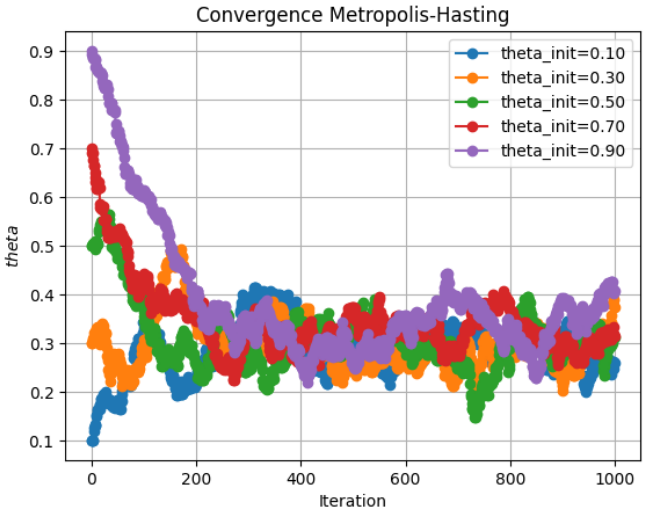
\includegraphics[width=\linewidth]{plots/output_univar.png}
    \caption{Convergence of markov chains from different initial values}
    \label{fig:my_label}
\end{figure}
    
\subsection*{MCMC Bivariate case}

In the current study, we extend the Markov Chain Monte Carlo (MCMC) framework to a bivariate case, addressing the scenario where two dependent probabilities are to be inferred. We denote the two observations as \( y = [y_1, y_2] \) and the corresponding parameters as \( \theta = [\theta_1, \theta_2] \). Each observation is assumed to be binomially distributed with \( y_1 \) trials and \( y_2 \) trials, leading to \( y_1 | \theta \sim \text{bin}(n_1, \theta_1) \) and \( y_2 | \theta \sim \text{bin}(n_2, \theta_2) \), respectively.

Given observations $y = [y_1, y_2]$ and parameters $\theta = [\theta_1, \theta_2]$, with $y_1 \sim \text{bin}(n_1, \theta_1)$ and $y_2 \sim \text{bin}(n_2, \theta_2)$, the Bayesian framework is applied to infer the posterior distributions of $\theta_1$ and $\theta_2$.


Prior :
\[f(\theta) = f(\theta_1) \times f(\theta_2)\]

likelihood :
\[
L(\theta_1, \theta_2 | y_1, y_2) = \binom{n_1}{y_1} \theta_1^{y_1} (1 - \theta_1)^{n_1-y_1} \binom{n_2}{y_2} \theta_2^{y_2} (1 - \theta_2)^{n_2-y_2}.
\]

Posterior :
\[
f(\theta | y) \propto f(\theta) \times L(\theta | y).
\]

Proposal distribution :
\[\theta' | \theta \sim \text{Multivariate Normal}, \text{mean} = \theta\]

The prior distribution for \( \theta \) is factored into the priors for \( \theta_1 \) and \( \theta_2 \), implying a belief in the independence of the two parameters a priori, \( f(\theta) = f(\theta_1) \times f(\theta_2) \).

The likelihood function \( L(\theta_1, \theta_2 | y_1, y_2) \) is constructed from the product of two binomial likelihoods, reflecting the probability of observing \( y_1 \) and \( y_2 \) given \( \theta_1 \) and \( \theta_2 \), respectively.

The posterior distribution \( f(\theta | y) \) is then proportional to the product of the prior distribution and the likelihood function. This proportional relationship is a result of Bayes' theorem, which updates our beliefs about the parameters \( \theta_1 \) and \( \theta_2 \) in light of the observed data \( y_1 \) and \( y_2 \).

To explore the posterior distribution, we propose new candidate values of \( \theta \) from a multivariate normal distribution with the mean equal to the current estimate of \( \theta \). This proposal mechanism accounts for the potential correlation between \( \theta_1 \) and \( \theta_2 \) in the posterior distribution, which is particularly relevant in bivariate or multivariate cases where parameters may not be independent.

The below plots show the convergence of markov chains for \( \theta_1 \) and \( \theta_2 \) for the meropolis hastings algorithm

In the above example the Metropolis Hastings algorithm is used to estimate the joint posterior distribution of \( \theta_1 \) and \( \theta_2 \).At each step, a candidate parameter vector \( \theta_{\text{prop}} \) is proposed by adding a bivariate normal perturbation to the current parameter estimate \( \theta_{\text{current}} \). This perturbation ensures a random walk that explores the parameter space around the current estimate.

The proposed parameters are accepted if they fall within the valid interval \([0, 1]\) for both dimensions, ensuring that the parameters remain within the bounds of probability values. The acceptance ratio \( \alpha \), computed as the ratio of the proposed and current probabilities (prior times likelihood), governs the transition between states. If a uniformly random number is less than \( \alpha \), the proposed parameters are accepted, updating \( \theta_{\text{current}} \) to \( \theta_{\text{prop}} \), and are otherwise discarded.

The result is a sequence of \( \theta \) values that represent samples from the joint posterior distribution, providing insights into the probable values of the parameters given the observed data and the specified model.

\begin{figure}[htbp]
    \centering
    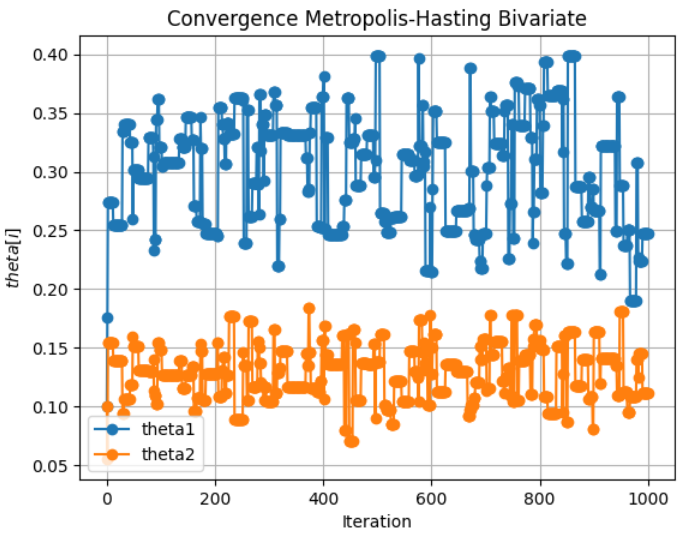
\includegraphics[width=\linewidth]{plots/output_bivar1.png}
    \caption{Convergence of markov chains for \( \theta_1 \) and \( \theta_2 \)}
    \label{fig:my_label}
\end{figure}
\begin{figure}[htbp]
    \centering
    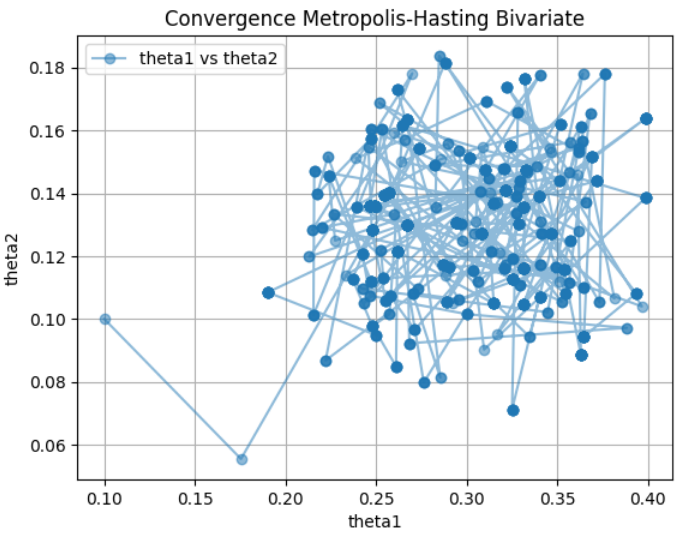
\includegraphics[width=\linewidth]{plots/output_bivar2.png}
    \caption{Convergence of metroplis chains for \( \theta_1 \) vs \( \theta_2 \)}
    \label{fig:my_label}
\end{figure}


\subsection*{MCMC Multivariate case}
In our research, we perform a Bayesian analysis using Markov Chain Monte Carlo (MCMC) on a dataset pertaining to vehicular stopping distances. The dataset comprises two variables: the speed of various vehicles and their corresponding stopping distances. We model the stopping distance as a linear function of speed, encapsulated by the equation \( y = ax + b + \varepsilon \), where \( \varepsilon \) is a normally distributed error term with mean zero and variance \( \sigma^2 \).

We define our parameter vector \( \theta = [a, b, \sigma] \) and express the likelihood of observing the data \( Y = [y_1, y_2, \ldots, y_n] \) given the speeds \( X = [x_1, x_2, \ldots, x_n] \) as a product of normal probability density functions. This reflects our assumption that the errors in the stopping distances follow a normal distribution.

Likelihood:
\[
L(\theta | X, Y) = \prod_{i=1}^{n} \frac{1}{\sqrt{2\pi\sigma^2}} \exp \left( -\frac{(y_i - ax_i - b)^2}{2\sigma^2} \right)
\]

To facilitate computation and to avoid numerical overflow issues, we employ the logarithm of the likelihood function, which transforms the product of exponentials into a summation of exponents. The log-likelihood is expressed as:
\[
\log L(\theta | X, Y) = \sum_{i=1}^{n} \left[ -\frac{1}{2} \log(2\pi\sigma^2) - \frac{(y_i - ax_i - b)^2}{2\sigma^2} \right].
\]

Our priors for \( a \) and \( b \) are modeled as normal distributions centered around zero, indicating no prior preference for the direction of the relationship between speed and stopping distance. For \( \sigma \), we employ a gamma prior, which is a common choice for a scale parameter such as the standard deviation in a normal distribution. The log-prior, thus, is a sum of the log-priors for \( a \), \( b \), and \( \sigma \):
\[
\log f(\theta) = \log f_{\mathcal{N}}(a) + \log f_{\mathcal{N}}(b) + \log f_{\text{gamma}}(\sigma).
\]

In the MCMC simulation, we propose new parameters \( \theta' \) using a multivariate normal distribution with a mean equal to the current estimate \( \theta \), allowing for the exploration of the parameter space. The acceptance probability \( \alpha \) is determined by the change in the log-likelihood and the log-prior from the current to the proposed parameters. If \( \alpha \) exceeds a random draw from a uniform distribution, we accept \( \theta' \), updating our parameter estimates; otherwise, we retain our current parameters.

In the above example, the Metropolis-Hastings algorithm is employed to estimate the posterior distribution of the parameters \( a \), \( b \), and \( \sigma \) in a linear regression model. The algorithm generates a sequence of parameter vectors that approximate the joint posterior distribution, allowing us to infer the relationship between speed and stopping distance in the dataset.

The sampling process begins by initializing the parameters of interest, \( a \), \( b \), and \( \sigma \), to reasonable starting values. These parameters encompass the slope, intercept, and standard deviation of the normal distribution for the error term, respectively.

At each iteration of the Metropolis-Hastings algorithm, candidate parameters, \( \theta_{\text{prop}} \), are generated via normal perturbations centered on the current parameter estimates, \( \theta_{\text{current}} \). These perturbations are applied individually to \( a \), \( b \), and \( \sigma \) with predefined standard deviations to regulate the step sizes of the random walk.

To maintain physical plausibility, proposed values for the standard deviation \( \sigma \) that are less than zero are outright rejected. This is because a negative standard deviation does not hold meaning in the context of our normal error model.

% The algorithm computes the log-likelihood and log-prior for both the current and proposed parameter sets. The log-likelihood is determined by the sum of the log probabilities from a normal distribution, given the observed stopping distances and the distances predicted by the linear model at the current speed values. The log-prior captures our initial beliefs about the parameter distributions: normal for \( a \) and \( b \), and a gamma distribution for \( \sigma \).

The acceptance ratio, \( \alpha \), is calculated as the exponential of the difference between the log-probabilities of the proposed and current parameters. If a uniformly drawn random number is less than \( \alpha \), the proposed parameters are accepted, updating \( \theta_{\text{current}} \) to \( \theta_{\text{prop}} \).

This stochastic acceptance criterion ensures that parameter updates are more likely when they result in higher posterior probability, thereby leading the chain towards regions of higher density in the parameter space. Through repeated iterations, this algorithm generates a sequence of parameter samples approximating the joint posterior distribution.

After many iterations, the algorithm yields an ensemble of parameter values that represent samples from the posterior distribution. These samples can then be used to infer the most probable estimates for the slope and intercept of the regression line, along with the standard deviation of the errors, thereby characterizing the relationship between speed and stopping distance.

\begin{figure}[htbp]
    \centering
    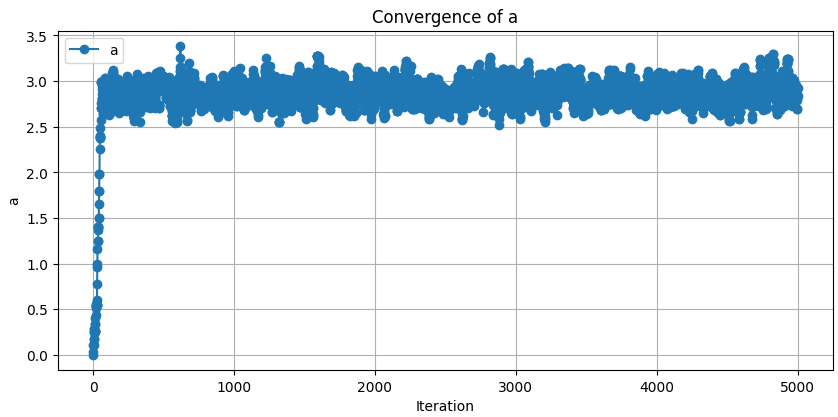
\includegraphics[width=\linewidth]{plots/output_multivar_1.png}
    \caption{Convergence of markov chains for \( a \)}
    \label{fig:my_label}
\end{figure}

\begin{figure}[htbp]
    \centering
    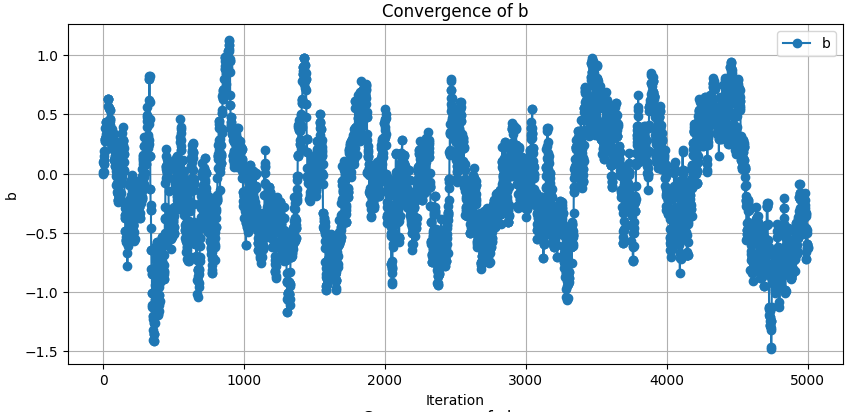
\includegraphics[width=\linewidth, height= 5cm]{plots/output_multivar_2.png}
    \caption{Convergence of markov chains for \( b \)}
    \label{fig:my_label}
\end{figure}

\begin{figure}[htbp]
    \centering
    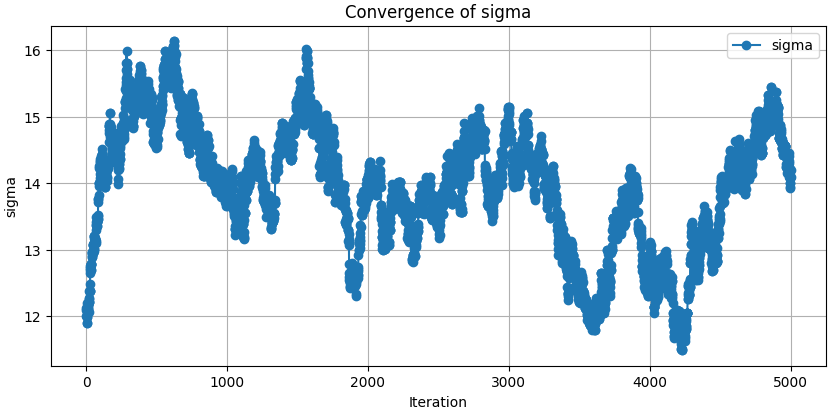
\includegraphics[width=\linewidth, height= 4cm]{plots/output_multivar_3.png}
    \caption{Convergence of metroplis chains for \(\sigma\)}
    \label{fig:my_label}
\end{figure}

\begin{figure}[htbp]
    \centering
    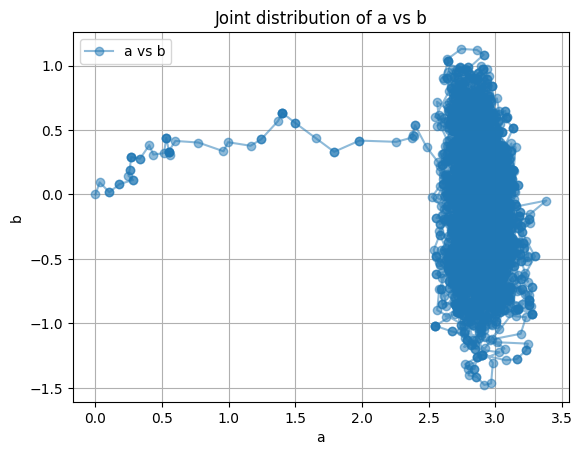
\includegraphics[width=\linewidth]{plots/output_multivar_4.png}
    \caption{Joint distribution of \(a\) and \(b\)}
    \label{fig:my_label}
\end{figure}

\begin{figure}[htbp]
    \centering
    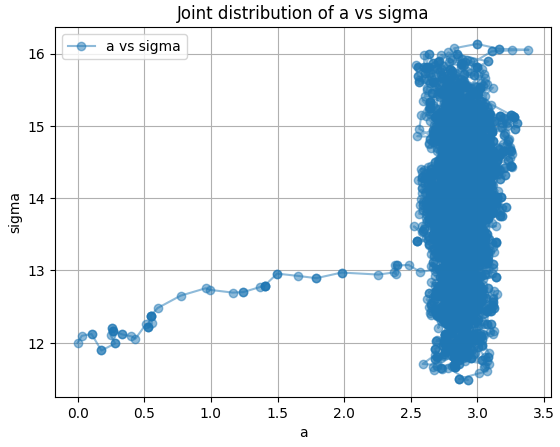
\includegraphics[width=\linewidth]{plots/output_multivar_5.png}
    \caption{Joint distribution of \(a\) and \(\sigma\)}
    \label{fig:my_label}
\end{figure}

\begin{figure}[htbp]
    \centering
    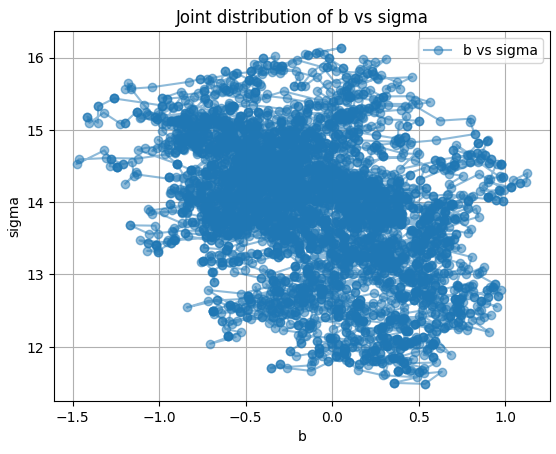
\includegraphics[width=\linewidth]{plots/output_multivar_6.png}
    \caption{Joint distribution of \(b\) and \(\sigma\)}
    \label{fig:my_label}
\end{figure}

The histogram visualization for posteriors of the parameters \( a \), \( b \), and \( \sigma \) provides insights into the probable values of these parameters given the observed data. The histograms represent the distribution of each parameter, with the x-axis denoting the parameter values and the y-axis indicating the frequency of occurrence. These visualizations offer a summary of the posterior distributions, highlighting the central tendency and variability of the parameter estimates.

\begin{figure}[htbp]
    \centering
    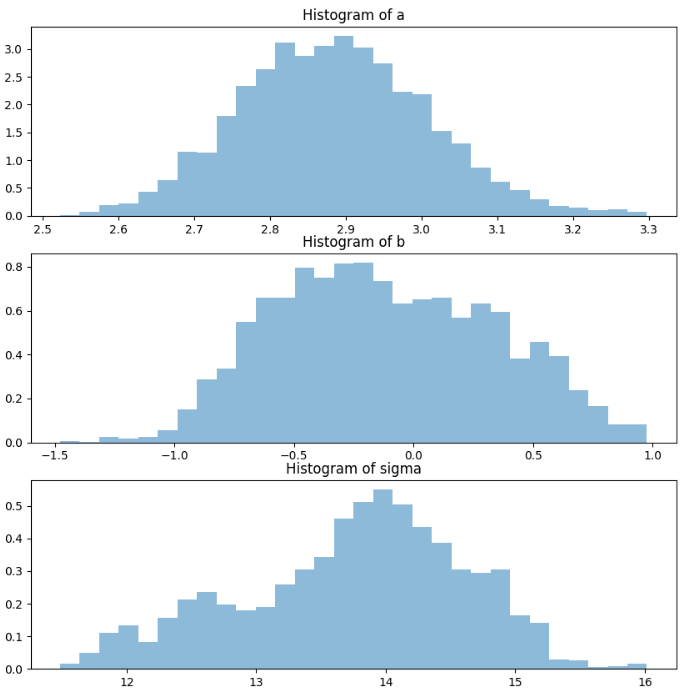
\includegraphics[width=\linewidth, height= 11cm]{plots/output_multivar_7.png}
    \caption{Histograms of the posterior distributions of \(a\), \(b\), and \(\sigma\)}
    \label{fig:my_label}
\end{figure}

\begin{figure}[htbp]
    \centering
    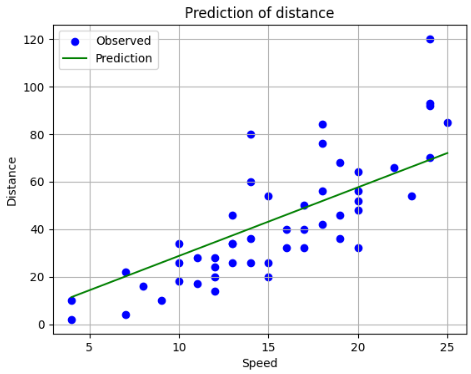
\includegraphics[width=\linewidth, height= 7cm]{plots/output_multivar_8.png}
    \caption{Prediction of stopping distances based on the linear model}
    \label{fig:my_label}
\end{figure}
\section{Conclusion}
The Bayesian inferential framework coupled with the Metropolis-Hastings algorithm has been shown to be an effective approach for the analysis of complex statistical models, especially in scenarios burdened with high dimensionality. In this study, we successfully applied these methodologies to the problem of estimating vehicle stopping distances as a function of speed. By carefully selecting priors and constructing a likelihood function reflective of the assumed normal distribution of errors, we have utilized the Metropolis-Hastings algorithm to generate an ensemble of parameter samples. These samples allowed us to draw inferences about the slope, intercept, and variability of the regression line governing the relationship between speed and stopping distance. The convergence of the Markov chains from multiple initial values demonstrates the robustness of our approach and provides a solid foundation for the reliability of MCMC methods in statistical inference. The results underscore the utility of Bayesian analysis and MCMC in solving complex problems where traditional methods may falter due to the curse of dimensionality.


{
    \small
    \nocite{*}
    % \bibliographystyle{ieeenat_fullname}
    % \bibliography{main}
    
}

% WARNING: do not forget to delete the supplementary pages from your submission 
% \input{sec/X_suppl}

\begin{thebibliography}{9}

    \bibitem{fish510}
    \textit{Introduction to Bayesian Statistics}.
    Available online: \url{https://www.webpages.uidaho.edu/fish510/pdf/bayestian.pdf} 
    
    \bibitem{ieee5767395}
    AuthorLastName, AuthorFirstName. 
    \textit{Title of the IEEE Paper}.
    Journal Name, volume, number, pages, year.
    Available online: \url{https://ieeexplore.ieee.org/stamp/stamp.jsp?tp=&arnumber=5767395&tag=1}
    
    \bibitem{wiki_metropolis}
    \textit{Metropolis–Hastings algorithm - Wikipedia}.
    Available online: \url{https://en.wikipedia.org/wiki/Metropolis\%E2\%80\%93Hastings_algorithm}
    
    \bibitem{mlgcam_rasmussen}
    Rasmussen, Carl Edward; Ghahramani, Zoubin.
    \textit{Gaussian Processes in Machine Learning}.
    2003.
    Available online: \url{https://mlg.eng.cam.ac.uk/pub/pdf/RasGha03.pdf}
    
    \end{thebibliography}
    
    


\end{document}